%\begin{enumerate}[label=\thesubsection.\arabic*.,ref=\thesubsection.\theenumi]
%\numberwithin{equation}{enumi}

\item
For a unity feedback system shown in  Fig.  \ref{fig:ee18btech11038_flow}, having transfer function given below in eq \ref{eq:ee18btech11038_tf}.  Design the value of gain K for $\brak{i}$ a gain margin of 38 dB. $\brak{ii}$ Phase margin of 40\degree. $\brak{iii}$ to yield maximum peak overshoot of 20 percent for a step input.

\begin{figure}[!ht]
	\begin{center}
		
		\resizebox{\columnwidth}{!}{%\begin{figure}
\tikzstyle{block} = [draw, fill=blue!20, rectangle, 
    minimum height=1cm, minimum width=1cm]
\tikzstyle{sum} = [draw, fill=blue!20, circle, node distance=1cm]
\tikzstyle{input} = [coordinate]
\tikzstyle{output} = [coordinate]
\tikzstyle{pinstyle} = [pin edge={to-,thin,black}]

% The block diagram code is probably more verbose than necessary
\begin{tikzpicture}[auto, node distance=2cm,>=latex']
    % We start by placing the blocks
    \node [input, name=input] {X(s)};
    \node [sum, right of=input] (sum) {};
    
    \node [block, right of=sum] (system) {$G(s)$ };
   
    % We draw an edge between the controller and system block to 
    % calculate the coordinate u. We need it to place the measurement block. 
    
    \node [output, right of=system] (output) {};
    \node [block, below of=system] (measurements) {1};

    % Once the nodes are placed, connecting them is easy. 
    \draw [draw,->] (input) -- node {$U(s)$} (sum);
    \draw [->] (sum) -- node {} (system);
    \draw [->] (system) -- node [name=y] {$Y(s)$}(output);
    \draw [->] (y) |- (measurements);
    \draw [->] (measurements) -| node[pos=0.99] {$-$} 
        node [near end] {} (sum);
\end{tikzpicture}
%\end{figure}}
	\end{center}
\caption{}
\label{fig:ee18btech11038_flow}
\end{figure}

\begin{align}
\label{eq:ee18btech11038_tf}
G\brak{s} &= \frac{K\brak{s+2}}{s\brak{s+3}\brak{s+4}\brak{s+5}}
\end{align}
\solution 

\begin{align}
\label{eq:ee18btech11038_TF(s)}
G\brak{s}H\brak{s} &=\frac{K\brak{s+2}}{s\brak{s+3}\brak{s+4}\brak{s+5}}
\end{align}
Name-
\begin{align}
\label{eq:ee18btech11038_T(s)}
T\brak{s} &= \frac{\brak{s+2}}{s\brak{s+3}\brak{s+4}\brak{s+5}}
\end{align}
Assuming positive value of K. Gain -
\begin{align}
\label{eq:ee18btech11038_gain}
      = 20log\brak{\abs{G\brak{s}H\brak{s}}}
    \\ \implies 20log\brak{K} +20log\abs{T\brak{s}}
\end{align}
Phase-
\begin{align}
\label{eq:ee18btech11038_phase}
      = \angle{G\brak{s}H\brak{s}}
    \\ \implies \angle{T\brak{s}}
\end{align}
 Thus value of K has - a) no effect on phase. b) linear effect on gain.




%\item $\brak{i}$ 
%\\
%\solution 
Given gain = 38dB,  The following code generates Bode plot of $T\brak{s}$ as shown in Fig \ref{fig:ee18btech11038_a}

\begin{lstlisting}
codes/ee18btech11038_a.py
\end{lstlisting}

\begin{figure}[!ht]
\centering
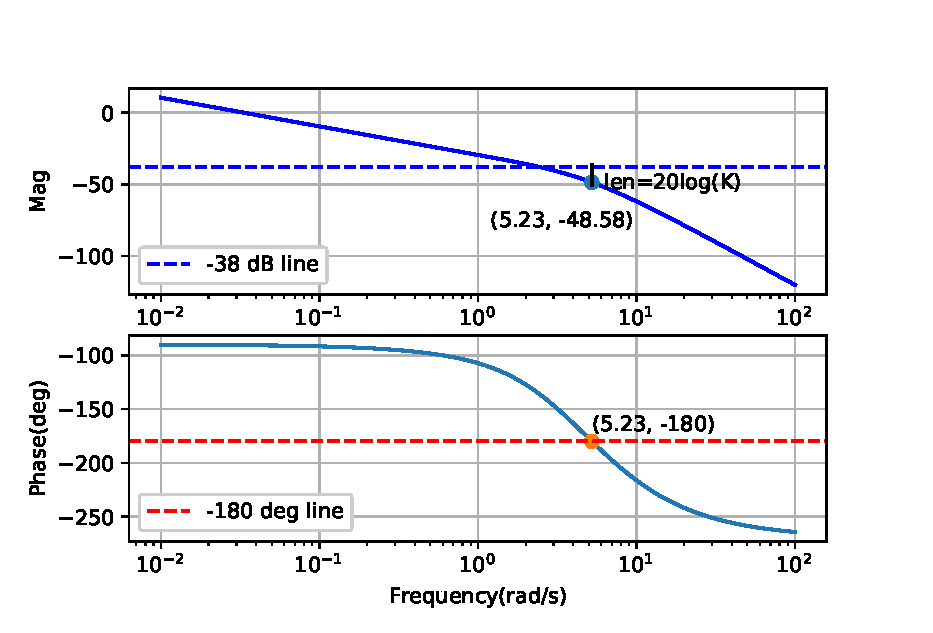
\includegraphics[width=\columnwidth]{./figs/ee18btech11038_a.eps}
\caption{Bode Plot of $T\brak{s}$}
\label{fig:ee18btech11038_a}
\end{figure}
Fig \ref{fig:ee18btech11038_a} shows how much the gain graph be slided to get -38 dB gain at $\omega_{pc}$.
From the graph $K = 3.38$
%\item 
Verify by substituting value of K obtained above. 
%\\
%\solution 
The following code generates Fig \ref{fig:ee18btech11038_vera}.

\begin{lstlisting}
codes/ee18btech11038_vera.py
\end{lstlisting}

\begin{figure}[!h]
\centering
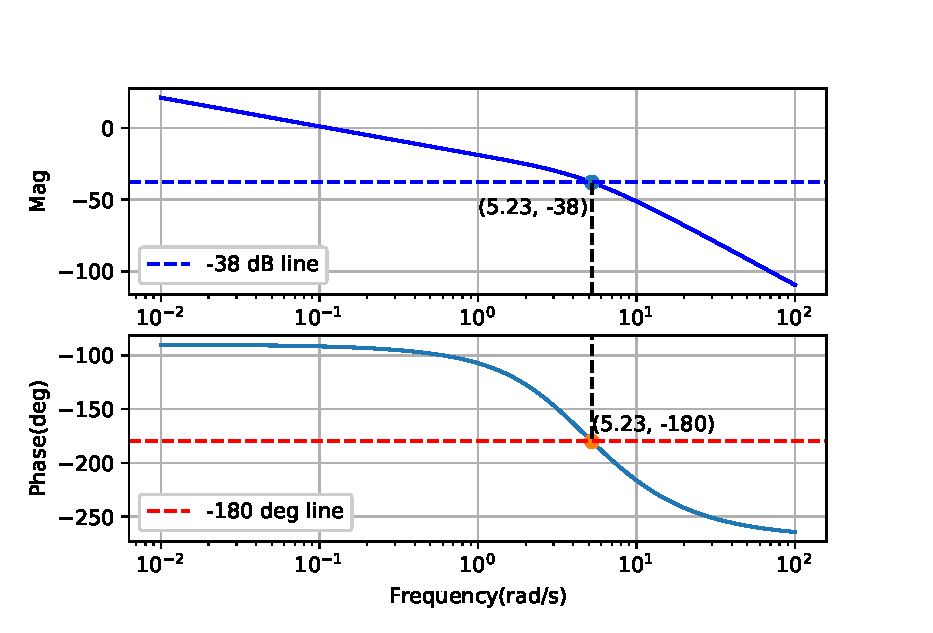
\includegraphics[width=\columnwidth]{./figs/ee18btech11038_vera.eps}
\caption{Bode Plot of $G\brak{s}$ with $K=3.38$ }
\label{fig:ee18btech11038_vera}
\end{figure}

%\item $\brak{i}$ 
Given PM = 40\degree
%\\
%\solution
\begin{align}
    phase\; at\; \omega_{gc} = -180\degree + PM
    \\
    \implies -140\degree
\end{align}
The following code generates Bode plot of $T\brak{s}$ to obtain $\omega_{gc}$ as shown in Fig \ref{fig:ee18btech11038_b}

\begin{lstlisting}
codes/ee18btech11038_b.py
\end{lstlisting}

\begin{figure}[!ht]
\centering
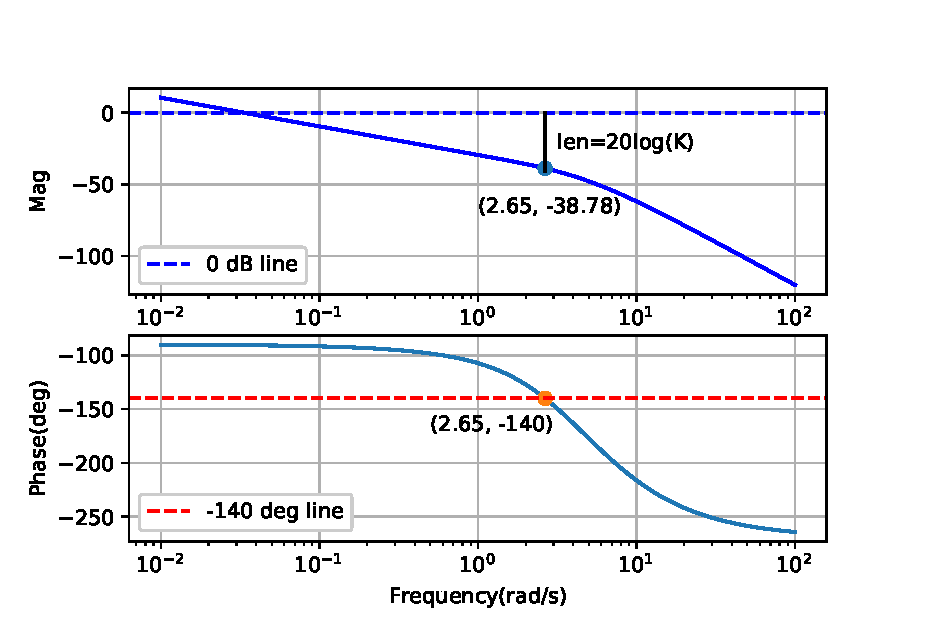
\includegraphics[width=\columnwidth]{./figs/ee18btech11038_b.eps}
\caption{Bode Plot of $T\brak{s}$}
\label{fig:ee18btech11038_b}
\end{figure}
Fig \ref{fig:ee18btech11038_b} shows how much the gain graph be slided to get 0 dB gain at $\omega_{gc}$.
From the graph $K =86.87$ 
%\item 
Verifying  by substituting value of K obtained above. 
%\\
%\solution 
The following code generates Fig \ref{fig:ee18btech11038_verb}.

\begin{lstlisting}
codes/ee18btech11038_verb.py
\end{lstlisting}

\begin{figure}[!h]
\centering
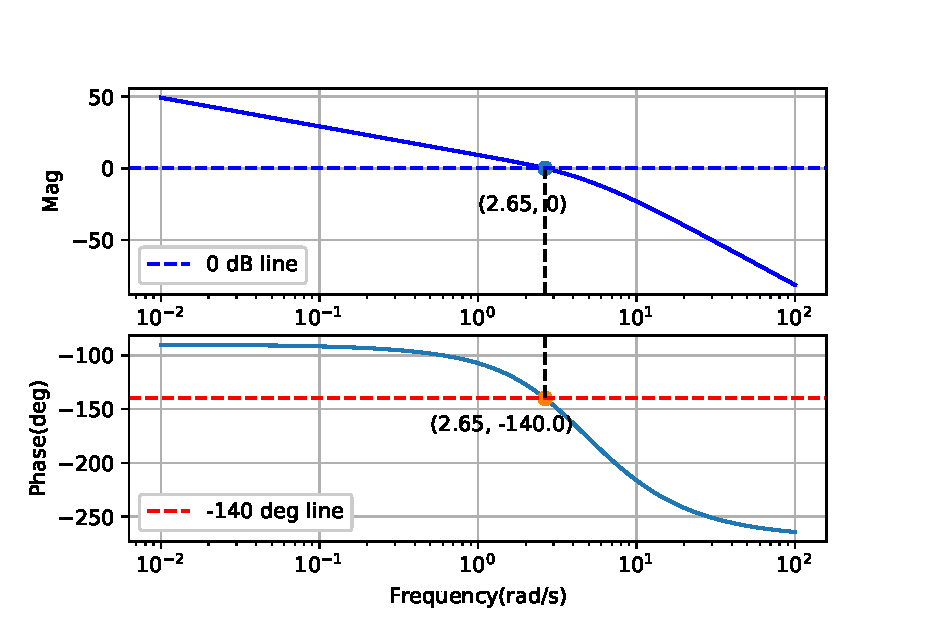
\includegraphics[width=\columnwidth]{./figs/ee18btech11038_verb.eps}
\caption{Bode Plot of $G\brak{s}$ with $K= 86.87$}
\label{fig:ee18btech11038_verb}
\end{figure}

%\item $\brak{iii}$ 
20 percent peak overshoot in step response.
%\\
%\solution 
\begin{align}
    \frac{G\brak{s}}{1+G\brak{s}} \quad \quad \quad\quad\quad
    \\
    \implies \frac{K\brak{s+2}}{s^4 + 12s^3 + 47s^2 + \brak{60+K}s + 2K} &= C\brak{s}
\end{align}
Step response-
\begin{align}
    \frac{K\brak{s+2}}{\brak{s}[s^4 + 12s^3 + 47s^2 + \brak{60+K}s + 2K]}
\end{align}
By final value theorem, steady state value-

\begin{align}
    \lim_{s \to 0} sC\brak{s} = \lim_{t \to \infty} c\brak{t} = 1
\end{align}
So the value at peak should be 1.2.
Now it is extremely difficult to find K  from the given data. Routh Hurwitz criteria only reveals that positive $K<156$.
Since it a fourth order system, there exist no explicit formula for peak time. Thus, trying a random value of K under the bound, then taking inverse Laplace and differentiating to get peak time and thus overshoot, is the only method that remains. Using trial and error K = 69.2 and Tpeak =1.19s

% \item 
Verify by substituting value of K. 
%\\
%\solution 
The following code generates Fig \ref{fig:ee18btech11038_os}.

\begin{lstlisting}
codes/ee18btech11038_os.py
\end{lstlisting}

\begin{figure}[!h]
\centering
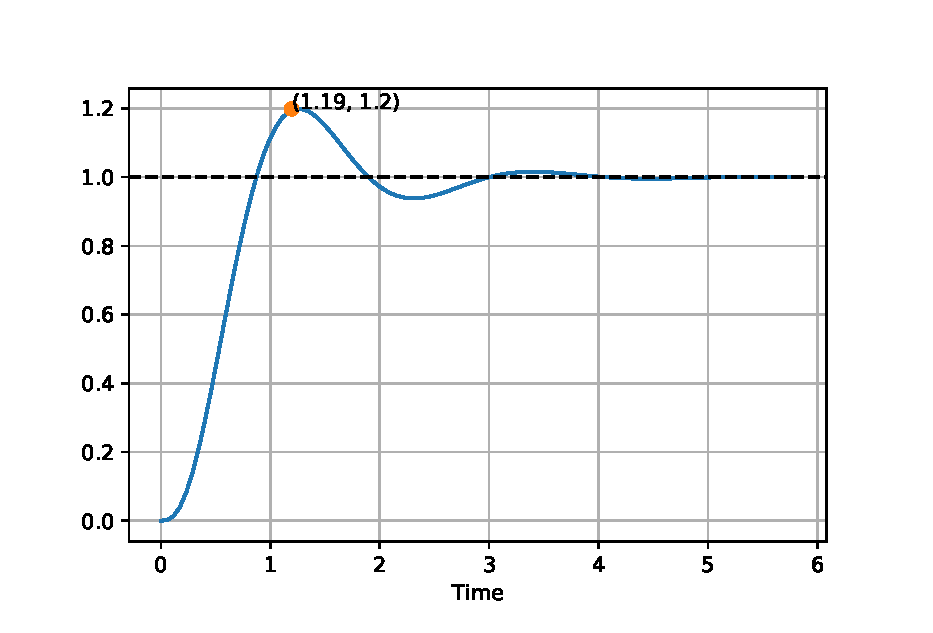
\includegraphics[width=\columnwidth]{./figs/ee18btech11038_os.eps}
\caption{Step Response of the sysytem for K = 69.2}
\label{fig:ee18btech11038_os}
\end{figure}
%\item 
Results in \ref{table:ee18btech11038_table}
\begin{table}[!ht]
\centering
%%%%%%%%%%%%%%%%%%%%%%%%%%%%%%%%%%%%%%%%%%%%%%%%%%%%%%%%%%%%%%%%%%%%%%
%%                                                                  %%
%%  This is the header of a LaTeX2e file exported from Gnumeric.    %%
%%                                                                  %%
%%  This file can be compiled as it stands or included in another   %%
%%  LaTeX document. The table is based on the longtable package so  %%
%%  the longtable options (headers, footers...) can be set in the   %%
%%  preamble section below (see PRAMBLE).                           %%
%%                                                                  %%
%%  To include the file in another, the following two lines must be %%
%%  in the including file:                                          %%
%%        \def\inputGnumericTable{}                                 %%
%%  at the beginning of the file and:                               %%
%%        \input{name-of-this-file.tex}                             %%
%%  where the table is to be placed. Note also that the including   %%
%%  file must use the following packages for the table to be        %%
%%  rendered correctly:                                             %%
%%    \usepackage[latin1]{inputenc}                                 %%
%%    \usepackage{color}                                            %%
%%    \usepackage{array}                                            %%
%%    \usepackage{longtable}                                        %%
%%    \usepackage{calc}                                             %%
%%    \usepackage{multirow}                                         %%
%%    \usepackage{hhline}                                           %%
%%    \usepackage{ifthen}                                           %%
%%  optionally (for landscape tables embedded in another document): %%
%%    \usepackage{lscape}                                           %%
%%                                                                  %%
%%%%%%%%%%%%%%%%%%%%%%%%%%%%%%%%%%%%%%%%%%%%%%%%%%%%%%%%%%%%%%%%%%%%%%



%%  This section checks if we are begin input into another file or  %%
%%  the file will be compiled alone. First use a macro taken from   %%
%%  the TeXbook ex 7.7 (suggestion of Han-Wen Nienhuys).            %%
\def\ifundefined#1{\expandafter\ifx\csname#1\endcsname\relax}


%%  Check for the \def token for inputed files. If it is not        %%
%%  defined, the file will be processed as a standalone and the     %%
%%  preamble will be used.                                          %%
\ifundefined{inputGnumericTable}

%%  We must be able to close or not the document at the end.        %%
	\def\gnumericTableEnd{\end{document}}


%%%%%%%%%%%%%%%%%%%%%%%%%%%%%%%%%%%%%%%%%%%%%%%%%%%%%%%%%%%%%%%%%%%%%%
%%                                                                  %%
%%  This is the PREAMBLE. Change these values to get the right      %%
%%  paper size and other niceties.                                  %%
%%                                                                  %%
%%%%%%%%%%%%%%%%%%%%%%%%%%%%%%%%%%%%%%%%%%%%%%%%%%%%%%%%%%%%%%%%%%%%%%

	\documentclass[12pt%
			  %,landscape%
                    ]{report}
       \usepackage[latin1]{inputenc}
       \usepackage{fullpage}
       \usepackage{color}
       \usepackage{array}
       \usepackage{longtable}
       \usepackage{calc}
       \usepackage{multirow}
       \usepackage{hhline}
       \usepackage{ifthen}



%%  End of the preamble for the standalone. The next section is for %%
%%  documents which are included into other LaTeX2e files.          %%
\else

%%  We are not a stand alone document. For a regular table, we will %%
%%  have no preamble and only define the closing to mean nothing.   %%
    \def\gnumericTableEnd{}

%%  If we want landscape mode in an embedded document, comment out  %%
%%  the line above and uncomment the two below. The table will      %%
%%  begin on a new page and run in landscape mode.                  %%
%       \def\gnumericTableEnd{\end{landscape}}
%       \begin{landscape}


%%  End of the else clause for this file being \input.              %%
\fi

%%%%%%%%%%%%%%%%%%%%%%%%%%%%%%%%%%%%%%%%%%%%%%%%%%%%%%%%%%%%%%%%%%%%%%
%%                                                                  %%
%%  The rest is the gnumeric table, except for the closing          %%
%%  statement. Changes below will alter the table's appearance.     %%
%%                                                                  %%
%%%%%%%%%%%%%%%%%%%%%%%%%%%%%%%%%%%%%%%%%%%%%%%%%%%%%%%%%%%%%%%%%%%%%%

\providecommand{\gnumericmathit}[1]{#1} 
%%  Uncomment the next line if you would like your numbers to be in %%
%%  italics if they are italizised in the gnumeric table.           %%
%\renewcommand{\gnumericmathit}[1]{\mathit{#1}}
\providecommand{\gnumericPB}[1]%
{\let\gnumericTemp=\\#1\let\\=\gnumericTemp\hspace{0pt}}
 \ifundefined{gnumericTableWidthDefined}
        \newlength{\gnumericTableWidth}
        \newlength{\gnumericTableWidthComplete}
        \newlength{\gnumericMultiRowLength}
        \global\def\gnumericTableWidthDefined{}
 \fi
%% The following setting protects this code from babel shorthands.  %%
 \ifthenelse{\isundefined{\languageshorthands}}{}{\languageshorthands{english}}
%%  The default table format retains the relative column widths of  %%
%%  gnumeric. They can easily be changed to c, r or l. In that case %%
%%  you may want to comment out the next line and uncomment the one %%
%%  thereafter                                                      %%
\providecommand\gnumbox{\makebox[0pt]}
%%\providecommand\gnumbox[1][]{\makebox}

%% to adjust positions in multirow situations                       %%
\setlength{\bigstrutjot}{\jot}
\setlength{\extrarowheight}{\doublerulesep}

%%  The \setlongtables command keeps column widths the same across  %%
%%  pages. Simply comment out next line for varying column widths.  %%
\setlongtables

\setlength\gnumericTableWidth{%
	70pt+%
	70pt+%
	70pt+%
0pt}
\def\gumericNumCols{3}
\setlength\gnumericTableWidthComplete{\gnumericTableWidth+%
         \tabcolsep*\gumericNumCols*2+\arrayrulewidth*\gumericNumCols}
\ifthenelse{\lengthtest{\gnumericTableWidthComplete > \linewidth}}%
         {\def\gnumericScale{\ratio{\linewidth-%
                        \tabcolsep*\gumericNumCols*2-%
                        \arrayrulewidth*\gumericNumCols}%
{\gnumericTableWidth}}}%
{\def\gnumericScale{1}}

%%%%%%%%%%%%%%%%%%%%%%%%%%%%%%%%%%%%%%%%%%%%%%%%%%%%%%%%%%%%%%%%%%%%%%
%%                                                                  %%
%% The following are the widths of the various columns. We are      %%
%% defining them here because then they are easier to change.       %%
%% Depending on the cell formats we may use them more than once.    %%
%%                                                                  %%
%%%%%%%%%%%%%%%%%%%%%%%%%%%%%%%%%%%%%%%%%%%%%%%%%%%%%%%%%%%%%%%%%%%%%%

\ifthenelse{\isundefined{\gnumericColA}}{\newlength{\gnumericColA}}{}\settowidth{\gnumericColA}{\begin{tabular}{@{}p{70pt*\gnumericScale}@{}}x\end{tabular}}
\ifthenelse{\isundefined{\gnumericColB}}{\newlength{\gnumericColB}}{}\settowidth{\gnumericColB}{\begin{tabular}{@{}p{70pt*\gnumericScale}@{}}x\end{tabular}}
\ifthenelse{\isundefined{\gnumericColC}}{\newlength{\gnumericColC}}{}\settowidth{\gnumericColC}{\begin{tabular}{@{}p{70pt*\gnumericScale}@{}}x\end{tabular}}

\begin{tabular}[c]{%
	b{\gnumericColA}%
	b{\gnumericColB}%
	b{\gnumericColC}%
	}

%%%%%%%%%%%%%%%%%%%%%%%%%%%%%%%%%%%%%%%%%%%%%%%%%%%%%%%%%%%%%%%%%%%%%%
%%  The longtable options. (Caption, headers... see Goosens, p.124) %%
%	\caption{The Table Caption.}             \\	%
% \hline	% Across the top of the table.
%%  The rest of these options are table rows which are placed on    %%
%%  the first, last or every page. Use \multicolumn if you want.    %%

%%  Header for the first page.                                      %%
%	\multicolumn{3}{c}{The First Header} \\ \hline 
%	\multicolumn{1}{c}{colTag}	%Column 1
%	&\multicolumn{1}{c}{colTag}	%Column 2
%	&\multicolumn{1}{c}{colTag}	\\ \hline %Last column
%	\endfirsthead

%%  The running header definition.                                  %%
%	\hline
%	\multicolumn{3}{l}{\ldots\small\slshape continued} \\ \hline
%	\multicolumn{1}{c}{colTag}	%Column 1
%	&\multicolumn{1}{c}{colTag}	%Column 2
%	&\multicolumn{1}{c}{colTag}	\\ \hline %Last column
%	\endhead

%%  The running footer definition.                                  %%
%	\hline
%	\multicolumn{3}{r}{\small\slshape continued\ldots} \\
%	\endfoot

%%  The ending footer definition.                                   %%
%	\multicolumn{3}{c}{That's all folks} \\ \hline 
%	\endlastfoot
%%%%%%%%%%%%%%%%%%%%%%%%%%%%%%%%%%%%%%%%%%%%%%%%%%%%%%%%%%%%%%%%%%%%%%

\hhline{|-|-|-|}
	 \multicolumn{1}{|p{\gnumericColA}|}%
	{\gnumericPB{\centering}\textbf{Specification}}
	&\multicolumn{1}{p{\gnumericColB}|}%
	{\gnumericPB{\centering}\textbf{Propsed}}
	&\multicolumn{1}{p{\gnumericColC}|}%
	{\gnumericPB{\centering}\textbf{Actual}}


	
\\
\hhline{|-|-|-|}
	 \multicolumn{1}{|p{\gnumericColA}|}%
	{\gnumericPB{\centering}Gain Margin}
	&\multicolumn{1}{p{\gnumericColB}|}%
	{\gnumericPB{\centering}38}
	&\multicolumn{1}{p{\gnumericColC}|}%
	{\gnumericPB{\centering}38.003}
	\\
	\hhline{|-|-|-|}
	 \multicolumn{1}{|p{\gnumericColA}|}%
	{\gnumericPB{\centering}Phase Margin}
	&\multicolumn{1}{p{\gnumericColB}|}%
	{\gnumericPB{\centering}40\degree}
	&\multicolumn{1}{p{\gnumericColC}|}%
	{\gnumericPB{\centering}40.001\degree}
	\\
	
\hhline{|-|-|-|}
	 \multicolumn{1}{|p{\gnumericColA}|}%
	{\gnumericPB{\centering}OS\%}
	&\multicolumn{1}{p{\gnumericColB}|}%
	{\gnumericPB{\centering}20\%}
	&\multicolumn{1}{p{\gnumericColC}|}%
	{\gnumericPB{\centering}19.86\%}
\\
\hhline{|-|-|-|}
\end{tabular}

\ifthenelse{\isundefined{\languageshorthands}}{}{\languageshorthands{\languagename}}
\gnumericTableEnd

\caption{Comparing the Proposed and Actual results}
\label{table:ee18btech11038_table}
\end{table}
%\end{enumerate}
